\documentclass[10pt,conference]{IEEEtran}
\ifCLASSOPTIONcompsoc
  % IEEE Computer Society needs nocompress option
  % requires cite.sty v4.0 or later (November 2003)
  \usepackage[nocompress]{cite}
\else
  % normal IEEE
  \usepackage{cite}
\fi

\IEEEoverridecommandlockouts

\usepackage{mathptmx}
\usepackage{graphicx}
\usepackage{times}
\usepackage{subfigure}
\usepackage{capt-of}
\usepackage{amsmath}
\usepackage{amssymb}
\usepackage{siunitx}
\usepackage{amsbsy}
\usepackage{MnSymbol}
\usepackage{url}
\usepackage{mathtools,xparse}
\usepackage{amsfonts}
\usepackage{color}
\usepackage{xfrac}

\renewcommand{\arraystretch}{1.2}

\def\wrt{w.\,r.\,t.~}
\def\eg{e.\,g.~}
\def\ie{i.\,e.}
\def\Dash{\nobreak\,---\penalty-500\,}

%\usepackage{bbm} 
\newcommand\id{\ensuremath{{I}}}
\newcommand\ev{\ensuremath{{E}}}

\newcommand{\code}[1]{\texttt{#1}}

\newcommand{\Var}{\operatorname{Var}}
\newcommand{\Cov}{\operatorname{Cov}}

\definecolor{gray}{rgb}{0.3,0.3,0.3}

\DeclarePairedDelimiter{\abs}{\lvert}{\rvert}
\DeclarePairedDelimiter{\norm}{\lVert}{\rVert}
\NewDocumentCommand{\normL}{ s O{} m }{%
  \IfBooleanTF{#1}{\norm*{#3}}{\norm[#2]{#3}}_{L_2(\Omega)}%
}

\newcommand{\defeq}{\vcentcolon=}
\newcommand{\eqdef}{\mathrel{\mathop=}:}

\newenvironment{descr}[1]{\list{}{%
  \setlength{\topsep}{0pt}
  \setlength{\itemsep}{0pt}
  \setlength{\parsep}{0pt}
  \setlength{\itemindent}{0pt}
  \settowidth{\labelwidth}{#1}
  \setlength{\labelsep}{2ex}
  \setlength{\leftmargin}{\parindent}
  \addtolength{\leftmargin}{\labelwidth}
  \addtolength{\leftmargin}{\labelsep}
  }}
  {\endlist}
\newcommand{\itemdesc}[1]{\item[#1\hspace*{\fill}]}



\begin{document}
\title{Towards an Efficient Data Assimilation in Physically-Based Medical Simulations}

%%\author{Nazim~Haouchine,~\IEEEmembership{Member,~IEEE,}
%%        Stephane~Cotin,~\IEEEmembership{Member,~IEEE,}
%%        Jeremie~Dequidt,~\IEEEmembership{Member,~IEEE,}
%%        Igor~Peterlik,~\IEEEmembership{Member,~IEEE,}
%%        Mario~Sanz~Lopez,~\IEEEmembership{Member,~IEEE,}
%%        Errwan~Kerien,~\IEEEmembership{Member,~IEEE,}
%%        and~Marie-Odile~Berger,~\IEEEmembership{Member,~IEEE,}% <-this % stops a space


\author{Igor~Peterlik and Anton\'{\i}n~Kl\'{\i}ma%
\IEEEcompsocitemizethanks{
\IEEEcompsocthanksitem Igor Peterlik is with the Institute of Computer Science, Masaryk University, Czech Republic, E-mail: peterlik@ics.muni.cz.
\IEEEcompsocthanksitem Anton\'{\i}n Kl\'{\i}ma is with the Faculty of Informatics, Masaryk University, Czech Republic.
\IEEEcompsocthanksitem Access to computing and storage facilities owned by parties and projects contributing to the National Grid Infrastructure MetaCentrum, provided under the programme "Projects of Large Infrastructure for Research, Development, and Innovations" (LM2010005), is greatly appreciated.
}% <-this % stops a space


\thanks{}}


\IEEEtitleabstractindextext{%
\begin{abstract}
Computer simulation of soft tissues is rapidly becoming an important aspect in medical training, pre-operative planning and intra-operative navigation.
Whereas in medical training, generic models are usually employed, both planing and navigation require patient-specific modeling. However, creating a patient-specific model is a challenging task, as many of the mechanical parameters of the organ tissues are unknown. One way of addressing the issue is to extend the deterministic simulation by methods based on stochastic modeling.

In this paper we focus on parameter estimation in models with large number of degrees of freedom based on a variant Kalman filtering. 
The main contribution of the paper is a detailed description of an integration of two advanced concepts of numerical modeling: on one side, 
we employ a state-of-the-art method of data assimilation based on reduced-order Kalman filtering in order to perform 
parameter estimation of a finite-element model of non-linear elasticity used in medical simulations. 

In order to assess the method, we present a preliminary evaluation of the accuracy of the parameter estimation as well as the performance 
using synthetic data with added noise. We also evaluate the parallelized version of the prediction phase and finally 
we describe further perspectives which, as we believe, will bring the data assimilation of models with many parameters 
closer to the real-time processing. 
\end{abstract}

\smallskip

% Note that keywords are not normally used for peerreview papers.
\begin{IEEEkeywords}
Data Assimilation, Kalman Filtering, Non-linear elasticity, Finite Element Method, Patient-specific Modeling
\end{IEEEkeywords}}


% make the title area
\maketitle


\IEEEdisplaynontitleabstractindextext

\IEEEpeerreviewmaketitle

\section{Introduction}
\label{s:intro}
In the last decade the importance of computer medical simulation in surgical training, pre-operative planning and intra-operative guidance has increased considerably. The recent advances show that the physics-based simulations are becoming capable of providing efficient improvements in laparoscopic as well as open surgery: e.g. the augmented-reality techniques employing a patient specific model built from the pre-operative data begin to play an important role in surgical navigation during laparoscopic surgery~\cite{haouchine2015impact}. Further, the medical simulations almost directly contribute to the actual boost in the area of interventional radiology, which provides an alternative for treatment of complicated pathologies. 

However, the successful employment of computer simulation in surgical navigation and planning necessitates patient-specific modeling: 
besides the geometrical aspects which often show significant inter-subject variability, correct patient-specific parametrization of the physical models is another crucial condition necessary to maintain required accuracy, reliability and robustness of models. Nevertheless, despite recent advances in non-invasive techniques such as MRI and ultrasound elastography, parametrization of tissue models remain a difficult and challenging task. 

One way of addressing the issue is to extend the deterministic simulation by methods based on stochastic modeling. The computer model itself thus becomes a part of an iterative process usually referenced as \emph{data assimilation} where the numerical model is employed in the prediction phase, while the observations of the simulated phenomena are used to correct the estimations of the parameters as well as the predicted~\cite{grewal2014kalman}. Naturally, when compared to a  the \emph{forward} simulation executed with given parametrization, the data assimilation methods based on the predictor-corrector schemes repeatedly invoking 
the model function for different parametrizations in each step are computationally much more expensive.

While the data assimilation techniques have been usually employed to deal with systems having a low number of both parameters and degrees of freedom (DoF), recently published methods such as reduced-order Kalman filtering~\cite{moireau2011reduced} open new possibilities allowing for the data assimilation to be applied to models with significantly larger number of parameters and DoFs. The novel methods open new horizons in stochastic modeling: a typical example of a possible scenario is an image-guided navigation of a surgical intervention such as a laparoscopic hepatectomy or partial nephrectomy, where the actual position of the tumor is predicted via physics-based simulation using the pre-operative data and intra-operative acquisitions represented for example by a flow captured by a laparoscopic camera or 2D slice scanned by an ultrasound probe. Since the accuracy of the prediction of the tumor position depends on a model which in turn depends on the tissue parameters such as elasticity of the tissue which moreover display high level of heterogeneity, data assimilation seems to be a promising tool combining the computer model with corresponding uncertainties related to its parametrization and the real procedure integrated into the correction process via observations.

Indeed, the scenario described above requires tremendously efficient methods of both the computer simulation and data assimilation, ideally achieving real-time 
performance. Although the existing methods are still far from this ambitious objective, novel mathematical methods in combination with 
advanced technologies of computer science such as parallelization and hardware acceleration already bring encouraging results.  

In this rather technical paper, we focus on the implementation of a data assimilation technique based on the reduced-order Kalman filtering for estimation of parameters of a soft-tissue model based on the finite element formulation of non-linear elasticity. The implementation is based on an integration of two state-of-the-art packages: the Simulation Open Framework Architecture (SOFA) which is an open-source package implementing advanced physics-based modeling methods focusing on real-time simulation in medicine, and Verdandi, an open-source library implementing the recently introduced data-assimilation schemes. We also describe the parallelization which is employed in order to speed up the prediction phase.

After giving the implementation details, we present a set of preliminary results demonstrating the capabilities of the new data assimilation framework. Using 
synthetic data for which the ground truth is known, we first assess the accuracy of the parameter estimation in two different scenarios. Then, we evaluate the performance of the actual implementation and report the impact of further optimizations based on parallelization. Finally, we discuss the results and provide further perspectives which should bring the data-assimilation of models with large number of parameters closer to the real-time scenario required in many applications related to image-guided and simulation-based intra-operative navigation.

\newcommand{\msa}{\mathcal{M}_1}
\newcommand{\msb}{\mathcal{M}_2}
\newcommand{\eexp}{E_\text{exp}}
\newcommand{\evar}{E_\text{var}}

\section{Methods}
\label{s:method}
In this section, we first focus on the method of data assimilation based on Kalman filter. 
Since this area of research is vast, we present only 
brief description of the related methods and refer the reader to a detailed introduction to
filtering methods available for example in~\cite{grewal2014kalman, welch2006introduction}. Then, we focus on the 
recently developed \emph{reduced-order} varian of the unscented Kalman filter which is in the core of our work. 
Finally, we describe the model of deformable objects 
based on the finite-element formulation of the elasticity problem. 

%%%%%%%%%%%%%%%%%%%%%%%%%%% KF:

\subsection{Data Assimilation Based on Kalman Filtering}
\label{sm:kalman}
One of the important data assimilation techniques is \emph{Kalman filtering},
%\footnote{The word \emph{filter} comes from the Kalman Filter's ability to filter out measurement noise, thus smoothing the simulation.} 
an algorithm first proposed by R. E. K\'{a}lm\'{a}n in 1960~\cite{kalman1960new}. The algorithm specifies a set of equations to be used for the prediction and correction steps. The reasoning behind the equations is based on a number of assumptions, under which the filter is in fact an optimal algorithm. Namely, these assumptions include  that the measurements are linked to the state of the model with linear equations, and that the state evolution of the model is also governed by linear equations.

The usefulness of Kalman filter was quickly recognized: the algorithm is especially suitable for real-time applications thanks to its low computational complexity as well as recursive nature. These features, highly desirable in many other applications, have encouraged the use of Kalman filter even for non-linear systems. To improve the algorithm's performance on these systems, a modification now known as \emph{extended Kalman filter} (EKF) was designed already in the 1960s. The EKF is based on the idea of linearizing the estimation around the current estimate in something akin to Taylor series \cite{welch2006introduction}. Notably, this modification retains the low computational demands of the original Kalman filter, although it requires mode intensive computations performed by the model which has to provide the Jacobian of the model function. 

The EKF and its numerous modifications have since claimed a central role in several applications such as the navigation systems and GPS. However, much like any approach based on Taylor series, this approach is particularly suitable when the time step is small enough; if only the first derivation is used, the function has to be \emph{almost linear} in the interval. If the non-linearity of the function dominates our computational capabilities (the step cannot be made small enough), the EKF is known to propagate the probability distributions of variables inaccurately, producing highly inaccurate results or even diverging~\cite{wan2000}.


%%%%%%%%%%%%%%%%%%%%%%%%%%% UKF:

\subsection{Unscented Kalman Filter}
\label{sm:UKF}
Whereas EKF is a rather straightforward application of basics of basic calculus and appeared shortly after the KF was designed, the \emph{Unscented Kalman Filter} (UKF) was designed by Julier and Uhlmann only in 1997 \cite{julier1997new}. The UKF is based on the idea that it is easier to approximate a probability distribution than it is to approximate a function.  The state estimate distribution is again approximated by a Gaussian random variable
%\footnote{A Gaussian random variable is nickname for a random variable with normal probability distribution.}
(GRV), but this GRV is represented by a set of sample points, called \emph{sigma points}. The sigma points, when propagated through the \emph{genuine} non-linear system, achieve third-order accuracy \cite{wan2000} for \emph{any} nonlinear system. Remarkably, the computational complexity of UKF is asymptotically equal to that of EKF. Detailed derivations of the filter and comparison to other methods can be found in~\cite{julier2004unscented,wan2000}.

The scenario considered here is governed by \emph{non-linear} stochastic equation:
\begin{equation*}
\mathbf{x}_{n+1} = f(\mathbf{x}_{n}) + \mathbf{w}_{n}\,,
\end{equation*}
where $\mathbf{x}_n \in \mathbb{R}^p$ is the state of the assimilated model. The measurement is given by
\begin{equation*}
\mathbf{z}_n = h(\mathbf{x}_{n}) + \mathbf{v}_{n}\,.
\end{equation*}
where $\mathbf{z}_n$ is usually referenced as the \emph{innovation} necessary for computation of the correction via Kalman gain.
Both the errors are again Gaussian with zero mean and with co-variance matrices $\mathbf{Q}$ and $\mathbf{R}$ respectively. 

The UKF makes use of \emph{sigma points}, and thereby evaluates the model using a number "nearby" states and inferring its view of the situation from all these results along with the observations. To specify the UKF, we thus first explain what sigma points are and how they are obtained. Thereafter the modified prediction and correction step equations are presented. 

%\subsubsection{Sigma points}
Consider a random variable $\mathbf{x} \in \mathbb{R}^p$ and the derived random variable $\mathbf{x}_f = f(\mathbf{x})$, where $f$ is nonlinear. Sigma points $\mathbf{x}^{[i]}$ together with their weights essentially represent a probability distribution on a finite number of "noised" state vectors. The distribution satisfies a number of assumptions, which ensure that (1) the distribution has the same mean and co-variance matrix as $\mathbf{x}$, and (2) the distribution accurately approximates that of the transformed variable $\mathbf{x_f}$. The accuracy is to the second order for arbitrary $\mathbf{x}$ , and to third order if $\mathbf{x}$ is Gaussian~\cite{wan2000}.

We refer to a set of $r$ points $\mathbf{x}^{[i]}$ with weights $\alpha_i$, where the points can be expressed by
\begin{equation*}
\mathbf{x}^{[i]} = \ev (X) + \tilde{\mathbf{x}}^{[i]} \,,
\quad
1 \leq i \leq r \,,
\end{equation*}
as \emph{sigma points} if the following criteria are simultaneously met:
\begin{flalign}
\label{SP1}
\sum\limits_{i=1}^{r} \alpha_i &=1 \,\\
\label{SP2}
\ev_\alpha (\mathbf{X^*}) \defeq \sum\limits_{i=1}^{r} \alpha_i \mathbf{x}^{[i]} &= \ev(\mathbf{x})\,\\
\label{SP3}
\Cov_\alpha (\mathbf{X^*})  \defeq \sum\limits_{i=1}^{r} \alpha_i (\mathbf{x}^{[i]}- \ev (\mathbf{x})) \cdot (\mathbf{x}^{[i]}- \ev (\mathbf{x})) ^{\sf T} &= \Cov (\mathbf{x})
\end{flalign}
Here, $\mathbf{X}^* = \begin{bmatrix} \mathbf{x}^{[0]} ... \mathbf{x}^{[r-1]} \end{bmatrix}$ denotes the \emph{sigma point matrix}.
Note that the sigma points themselves are \emph{not} random variables. Assuming Equations \ref{SP1}, \ref{SP2} and \ref{SP3} hold, the following expressions trivially hold:
\begin{flalign*}
\sum\limits_{i=1}^{r} \alpha_i \mathbf{\tilde{x}}^{[i]} &= \mathbf{0}\,\\
\sum\limits_{i=1}^{r} \alpha_i \mathbf{\tilde{x}}^{[i]} \cdot ( {\mathbf{\tilde{x}}^{[i]}} )^{\sf T} &= \Cov(\mathbf{x}) \,.
\end{flalign*}
It can also be shown that
\begin{flalign*}
\ev_\alpha  (\mathbf{X^*}) &= \ev (\mathbf{x}_f) + o\left( \ev (\norm{\mathbf{\tilde{x}}}^2)\right) \,,\\
\Cov_\alpha   (\mathbf{X^*}) &= \Cov (\mathbf{x}_f) + o\left( \ev (\norm{\mathbf{\tilde{x}}}^2)\right) \,,
\end{flalign*}
which is exactly what we expect from the sigma points.

The system of Equations \ref{SP1}, \ref{SP2} and \ref{SP3} has an infinite number of solutions, especially as the number of sigma points may be arbitrary. We  present the three most popular heuristics, in terms of their position relative to the mean. These relative positions are represented as columns $\mathbf{I}^{[i]}$ of matrix $I$.
\begin{itemize}
\item \emph{simplex sigma points}: This heuristic determines $r=p+1$ sigma points where $p$ is the dimension of the state vector. Also note that $r=p+1$ is the smallest possible number of sigma points. The sigma points $\mathbf{I}^{[i]}$ form a regular polyhedron of radius $\sqrt{p}$ and $\alpha_i = \sfrac{1}{p}$.
\item \emph{canonical sigma points}: This heuristic determines $r=2p$ sigma points. The points are located at $\mathbf{I}^{[i]} = -\mathbf{I}^{[i+p]}= \sqrt{p} \cdot \mathbf{e}_i$, where $\{\mathbf{e}_i\}$ is an orthonormal basis of $\mathbb{R}^p$, and $\alpha_i = \sfrac{1}{2p}$.
\item \emph{star sigma points}: This heuristic determines $r=2p+1$ sigma points, located at $\mathbf{I}^{[i]} = -\mathbf{I}^{[i+p]}= \sqrt{p} \cdot \mathbf{e}_i$ and at $\mathbf{I}^{[2p+1]}=\mathbf{0}$. The value of $\alpha$ is $\alpha_i = \sfrac{1}{2p+1}$.
\end{itemize}
%These herustics for sigma points are illustrated in two dimensions in Figure \ref{sigsalabim}.
% \begin{figure}[ht]
%     \centering
%     \includegraphics[width=1.0\textwidth]{sigma.png}
%     \caption{Sigma point choices in two dimensions about the cross (mean). \textbf{blue:} simplex. \textbf{green:} canonical. \textbf{red:} star.}
% \label{sigsalabim}
% \end{figure}
Given the choice of sigma points, the unscented Kalman filter is given by following sets of equations, divided into the prediction and correction phase:

\subsubsection{UKF --- Prediction Step}

\begin{flalign}
\label{sampling}
\mathbf{\hat{x}}_n^{[i]+} &= \mathbf{\hat{x}}_n^{+} + \sqrt{\mathbf{P}_{n}^{+}}I^{[i]} \,,\\
\mathbf{\hat{x}}_{n+1}^{-} &= \ev_\alpha (f(\mathbf{\hat{x}}^{*+}_n))\,,\\
\mathbf{P}_{n+1}^{-} &= \Cov_\alpha(f(\mathbf{\hat{x}}_n^{*+})) + \mathbf{Q} \,,
\end{flalign}
The step described by Equation \ref{sampling} is sometimes referred to as \emph{sampling} -- its output are sigma points for the current step. Thereafter, the model is applied to
the sigma points, and the mean and covariance of the probability distribution on them is determined and saved as \emph{a priori} estimates.

\subsubsection{UKF --- Correction Step}
\begin{flalign}
\mathbf{\hat{x}}_{n+1}^{[i]-} &= \mathbf{\hat{x}}_{n+1}^{-}  + \sqrt{\mathbf{P}_{n+1}^{-}}I^{[i]} \,,\\
\mathbf{{z}}_{n+1}^{[i]} &= h (\mathbf{\hat{x}}_{n+1}^{[i]-})  \,,\\
\mathbf{P}_{\alpha}^{\tilde{x} \tilde{z}} &= \Cov_\alpha (\mathbf{z}_{n+1}^*, \mathbf{z}_{n+1}^*) \,,\\
\mathbf{P}_{\alpha}^{\tilde{z}} &= \mathbf{R}_{n+1} + \Cov_\alpha (\mathbf{z}_{n+1}^*, \mathbf{z}_{n+1}^*)\,,\\
 \mathbf{\hat{K}}_{n+1} &=  \mathbf{P}_{\alpha}^{\tilde{x} \tilde{z}} \cdot (\mathbf{P}_{\alpha}^{\tilde{z}} )^{-1} \,,\\
\label{UKFup1}
 \mathbf{\hat{x}}_{n+1}^+ &=  \mathbf{x}_{n}^{-} +  \mathbf{\hat{K}}_{n+1}  (\mathbf{z}_{n+1} - \ev_\alpha(\mathbf{z}^*_{n+1}))\,,\\
\label{UKFup2}
 \mathbf{\hat{P}}_{n+1}^+ &=  \mathbf{\hat{P}}_{n+1}^- -  \mathbf{P}_{\alpha}^{\tilde{x} \tilde{z}} \cdot
 (\mathbf{P}_{\alpha}^{\tilde{z}} )^{-1} (\mathbf{P}_{\alpha}^{\tilde{x} \tilde{z}})^{\sf T}\,.
\end{flalign}
Here, the Eq. 8 represents the computation of \emph{innovation} given by the function $h$ requiring the observations of the 
modeled phenomenon. 


\begin{figure*}[t!]%
\centering%
\subfigure[]{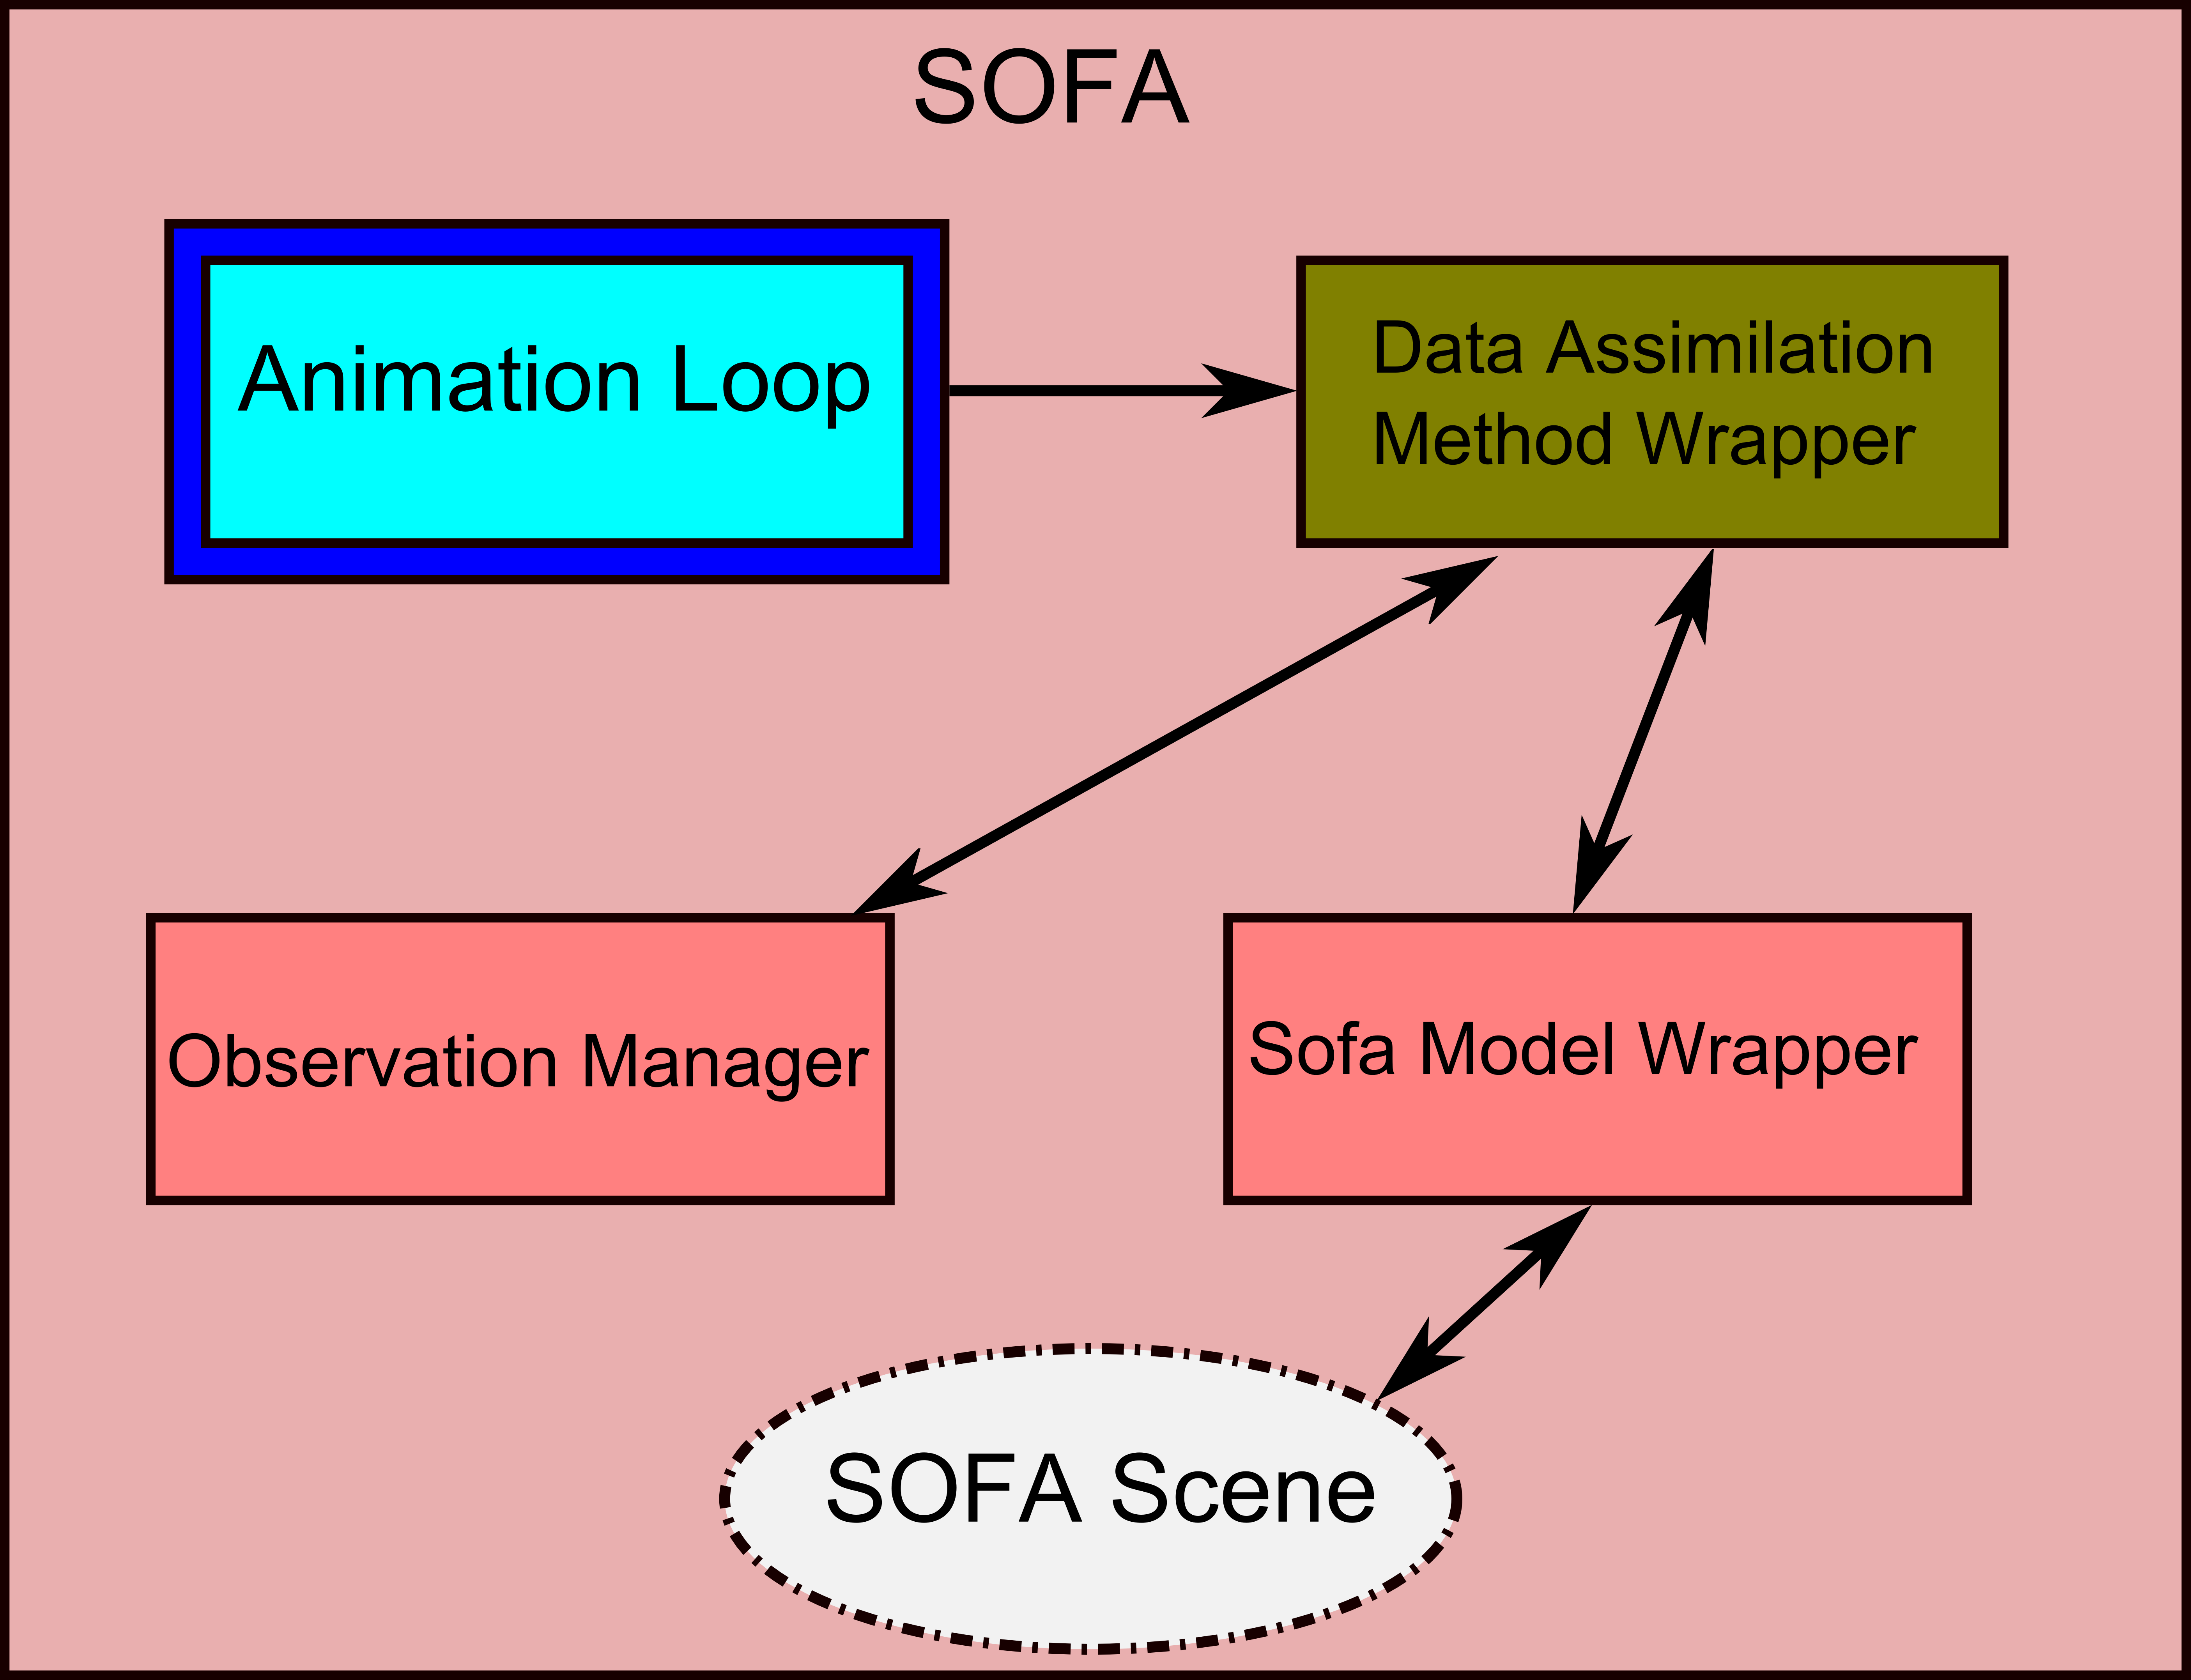
\includegraphics[height=4cm]{figs/integrationScheme1.png}}
\hfill
\subfigure[]{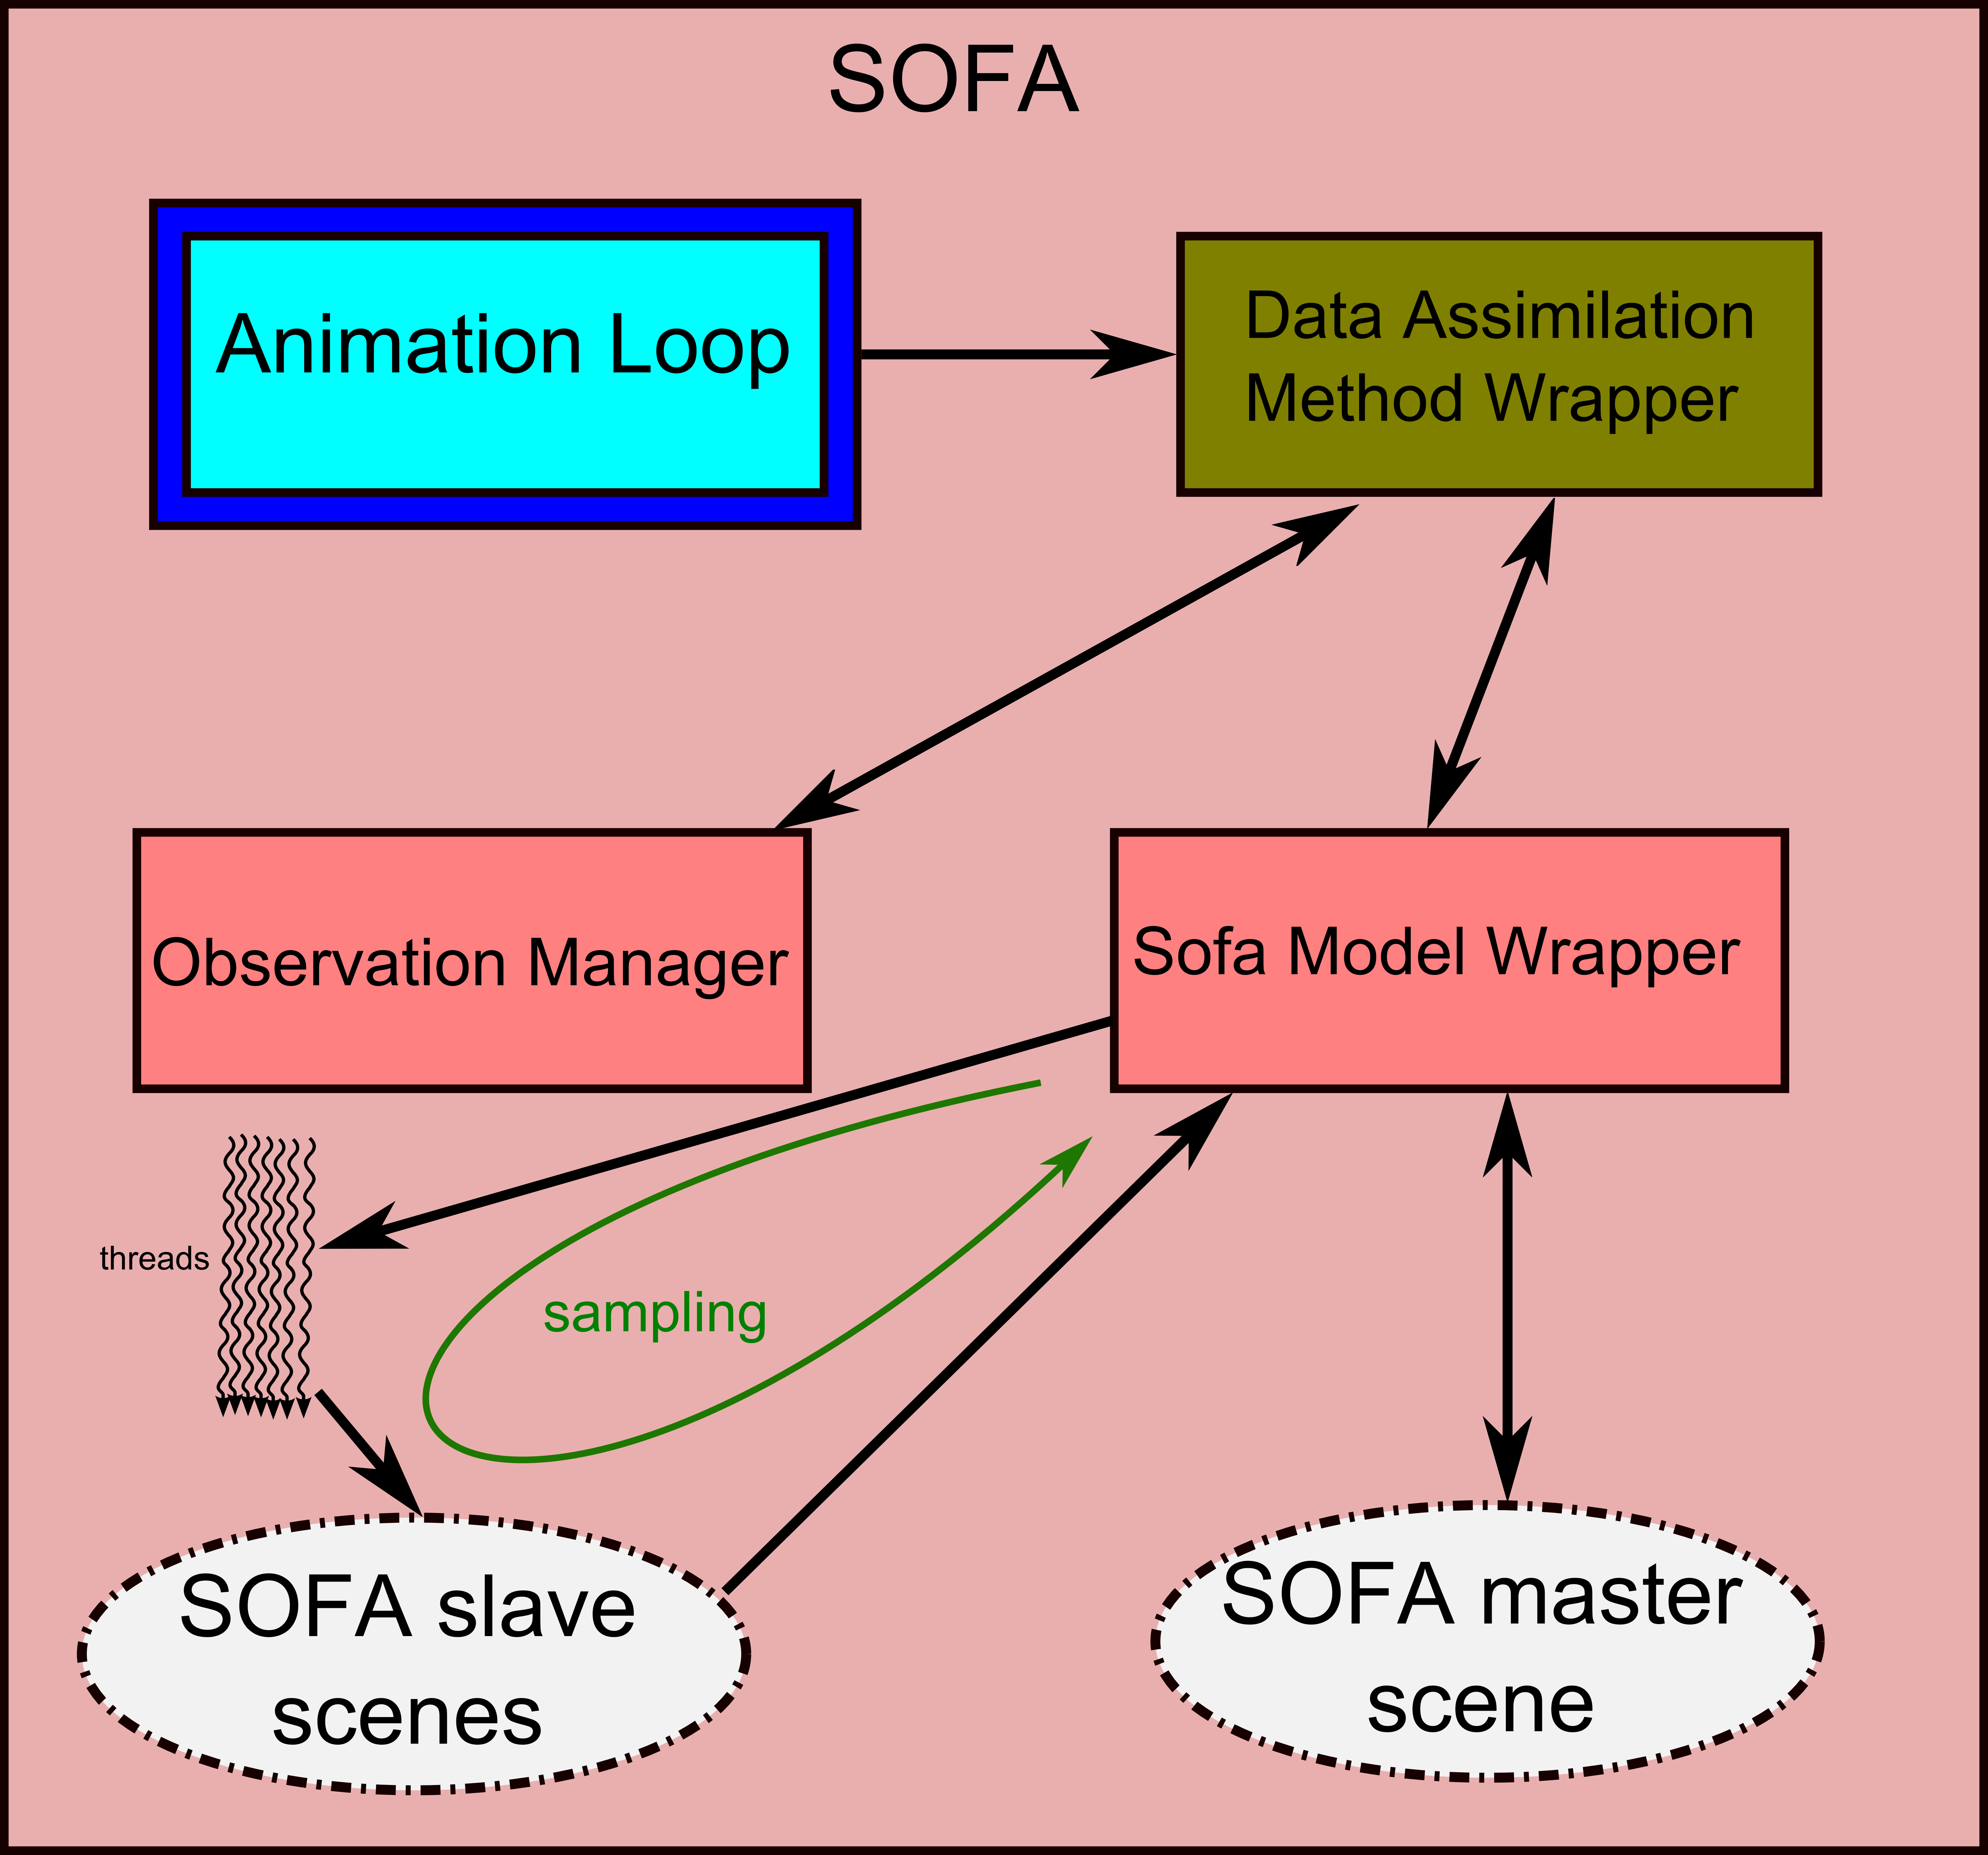
\includegraphics[height=4cm]{figs/integrationScheme2.png}}
\hfill
\subfigure[]{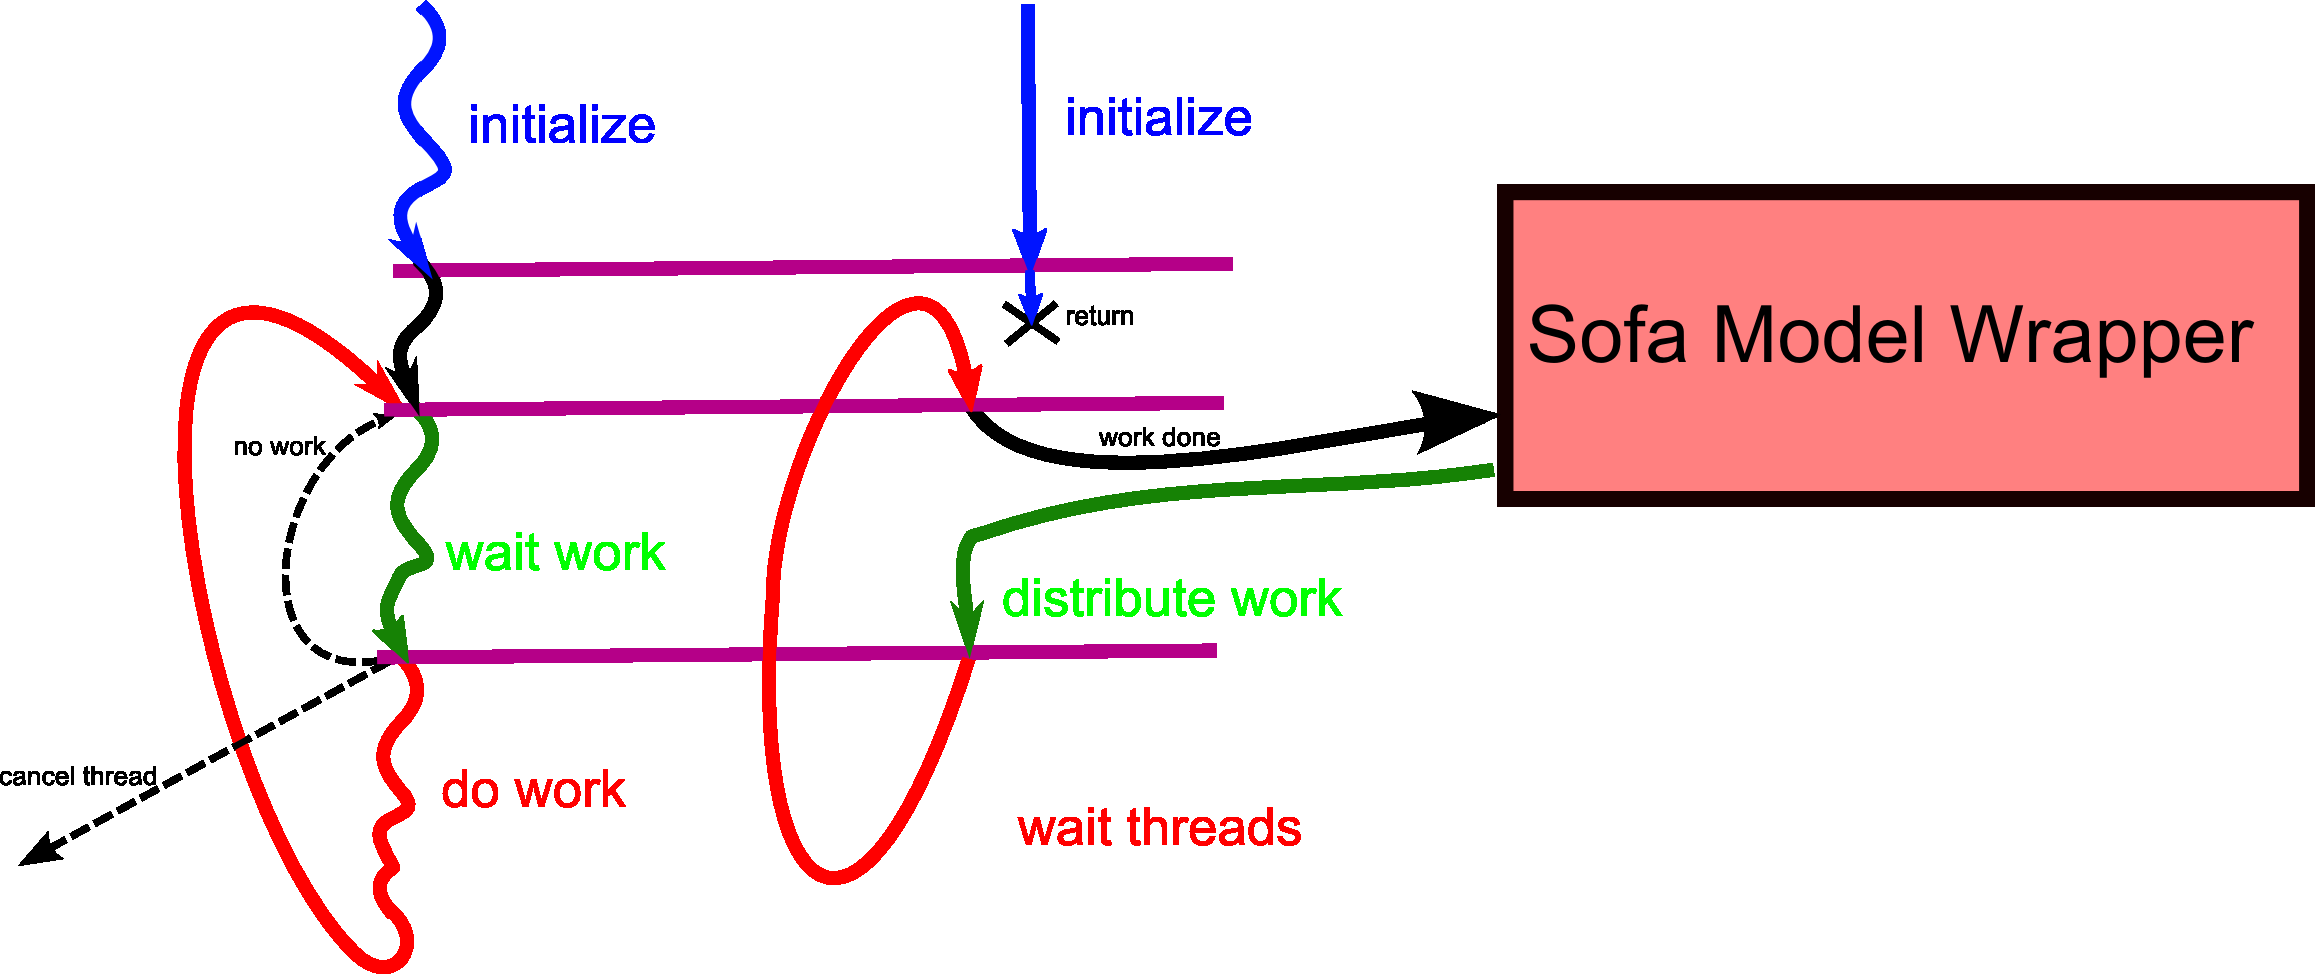
\includegraphics[width=.40\textwidth]{figs/parallelization.png}}
\caption{The schemes depict the integration of SOFA and Verdandi frameworks: (a) The sequential case where the ROUKF invokes the 
model function for each sigma point in a serial manner. (b) The parallel implementation where several instances of the model 
exist and can be evaluated concurrently for different parametrizations. (c) Scheme of the master-slave implementation of the parallel model 
wrapper, where the master thread distribute the work among slaves which execute the actual simulation step for given parametrization.}%
\label{f:integration}
\end{figure*}

\subsection{Reduced-Order Unscented Kalman Filter}
\label{sm:ROUKF}

One of the possible optimizations for large-dimensional systems is based on the observation that the matrix $\mathbf{P}$ is often of reduced rank $d \ll p$. We can then factorize the matrix $\mathbf{P}$ as
\begin{equation*}
\mathbf{P} = \mathbf{L} \mathbf{U}^{-1}\mathbf{L}^{\sf T} \,,
\end{equation*}
where $\mathbf{U}$ is a $d \times d$ invertible matrix -- this matrix then represents the uncertainties in the system. By rewriting the Eq.~\ref{sampling} through \ref{UKFup2} in a way that avoids the direct computation of $\mathbf{P}$, the computational demands decrease considerably. The main benefit is avoiding direct computation of $\mathbf{P}^{-1}$ which, unlike other matrix operations, does not benefit from the sparsity of the matrices. This modification is called \emph{Reduced-order Unscented Kalman Filter} (ROUKF); a detailed description of ROUKF can be found in~\cite{moireau2011reduced}.

%Another room for improvement is the computation of the model step.
%\footnote{Arguably also the measurement step if it were sufficiently computationally intensive.}.
%In an ordinary forward simulation, the simulation steps are inherently sequential and the only room for parallelization is within the individual steps. On the %contrary, the UKF computes $r$ model steps at each simulation step. Considering that the state vector represents the degrees of freedom of the system, the UKF increases the computational complexity by a linear factor. 
%\footnote{For the considered sigma point heuristics featuring O(p) sigma points.}. 
%Furthermore, the computations on different model steps require no coordination --- the task is \emph{embarrassingly parallel} --- and the model step tends to be a rather expensive operation. These facts provide a strong reason to believe that parallelizing the model step computation could provide us with a highly scalable and substantial performance improvement.

\def\bp{\mathbf{p}}
\def\be{\mathbf{e}}
\def\bff{\mathbf{p}}
\def\bfo{\mathbf{p}}
\def\bu{\mathbf{u}}
\def\bx{\mathbf{x}}
\def\bK{\mathbf{A}}
\def\bt{\mathbf{t}}
\def\bR{\mathbf{R}}
\def\bO{\mathbf{O}}
\def\bB{\mathbf{B}}
\def\bL{\mathbf{L}}
\def\bJ{\mathbf{J}}
\def\bF{\mathbf{F}}
\def\br{\mathbf{r}}

\subsection{Model of Deformations}
\label{sm:model}
In this section we provide details about the model which is used in the prediction phase of the ROUKF filter, \ie\ the 
\emph{model function} $f(\mathbf{x})$ called repeatedly in Eq. 5.
In this paper, we consider a physically-based model of deformations which is usually employed for soft-tissue modeling 
in the context of medical simulations.
As we do not focus on the transient part of the deformation, we suppose a quasi-static simulation where 
the actual deformation is given by application of external forces. On the other hand, we aim at modeling large deformations correctly, since
during the surgical interventions, important displacements of tissue occur due to the action of surgical tools.

For this reason we have opted for a finite element method based on a co-rotational formulation introduced by Felippa in~\cite{Felippa2005}, which allows for
large displacements while relying on a linear expression of the stress-strain relationship.
%which respects the rotational invariance needed for correct rendering of large deformations.
The co-rotational approach is based on decomposition of the actual element configuration into rigid rotation and pure deformation, 
both being quantified \wrt~the initial position. More precisely, the actual position of the element nodes
determines the base of the element (given by three chosen adjacent edges), which is both rotated and deformed \wrt\ the initial base of the same element.
In order to extract the rotational component (denoted as $\bR_e$), a matrix decomposition such as polar, SVD or QR is needed;
in our method we employ the technique described in~\cite{Nesme2005}.
The matrix $\bR_\be$ is used to update the local stiffness matrix $\bK_\be$ of the element.
Therefore, via this element-wise rotations, the actual global stiffness matrix $\bK$ depends in each step on the actual deformation $\bu$
and the equation relating the external forces to the displacements can be written as
\begin{equation}
\bK(\bu) = \bfo
%\; \text{ with }  \; \bu = \bx - \bx^0
\label{eq:corotational}
\end{equation}
\noindent where $\bu$ is the vector of displacements and $\bfo$ gathers the applied external forces.
The system represented by Eq.~\ref{eq:corotational} cannot be 
resolved directly due to the non-linearity of $\bK$ \wrt\ $\bu$. Therefore, Newton-Raphson method is employed: 
the system is iteratively solved while in each iteration, linearized \emph{tangent stiffness matrix} $\frac{\partial\bK}{\partial\bu}$ must
be assembled and inverted.

In order to assemble the system matrix $\bK$ and its derivatives, it is necessary to determine mechanical parameters: in the corotational approach considered 
in this paper, the system is parametrized with Poisson's ratio $\nu\in\langle 0,0.5)$ which is the measure of the material compressibility, 
and Young's modulus $E$ [Pa] which quantifies the stiffness of the material. In the context of medical simulations, the Poisson's ratio
close to 0.5 is usually employed. On the other hand, the Young's modulus is a typical representative of a parameter which is patient specific
(as shown for example in~\cite{yeh2002elastic}), nevertheless, it impacts the accuracy of the model significantly.

As we deal with a quasi-static solution, we suppose that 
a sequence of applied external forces $\bfo^{(1)}, \bfo^{(2)}, \ldots, \bfo^{(s)}$ results in a sequence of state vectors
$\bx^{(1)}, \bx^{(2)}, \ldots, \bx^{(s)}$ where $\bx^{(k)} = \bx_0 + \bu^{(k)}$, $\bx_0$ being the vector corresponding to the undeformed initial 
configuration and $\bu^{(k)}$ the displacement computed in $k$-th step of the simulation using Eq.~\ref{eq:corotational}. 

In order to return to the data assimilation scenario, Eq.~\ref{eq:corotational} can be regarded as the model function which transforms 
the actual state of the system represented by the vector of positions $\bx^{(k)}$ into a new state $\bx^{(k+1)}$ as the applied forces
change from $\bfo^{(k)}$ to $\bfo^{(k+1)}$. Since the evaluation of the applied forces is usually smooth, 
the resolution of the non-linear system given by Eq.~\ref{eq:corotational} in step $(k+1)$ can be significantly 
improved by employing the state $\bx^{(k)}$ as the starting configuration of the Newton-Raphson iterative process. 

\begin{figure*}[th]%
\centering%
\subfigure[]{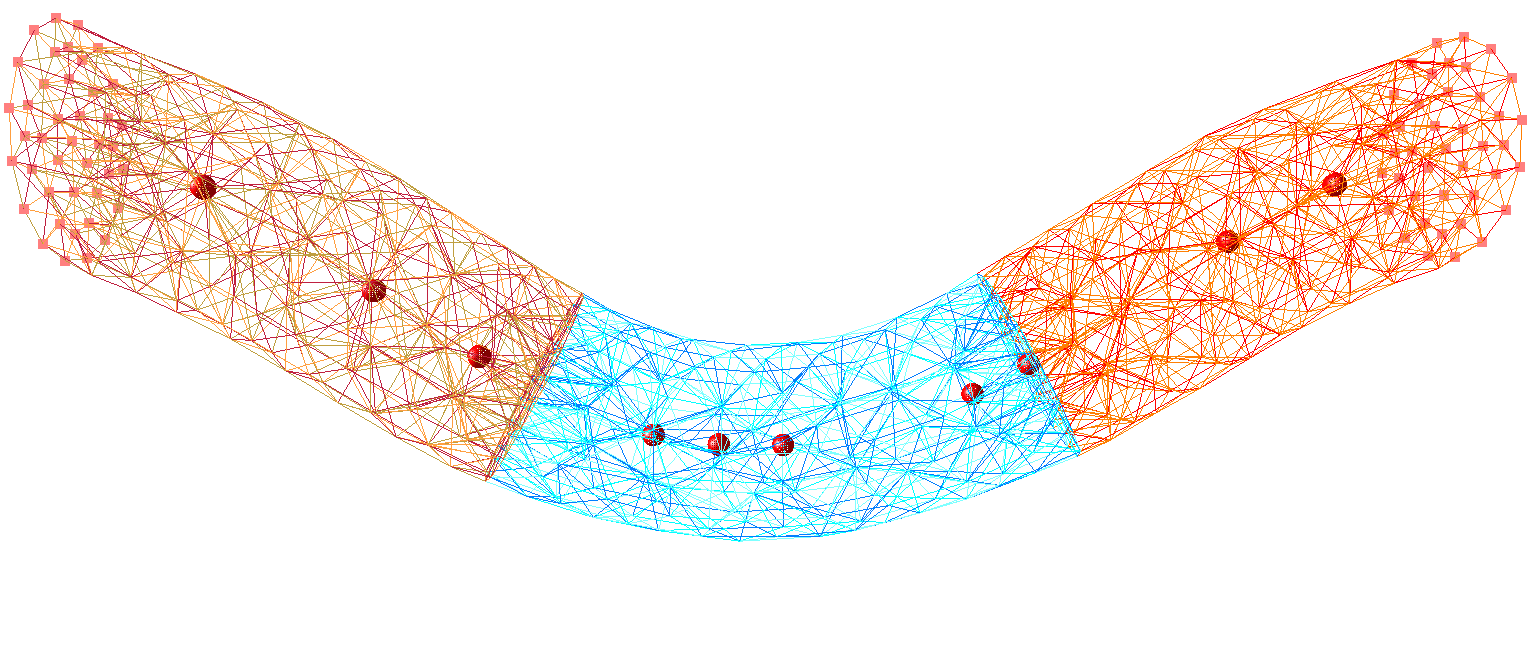
\includegraphics[width=.48\textwidth]{figs/cyl3screen.png}}
\hfill
\subfigure[]{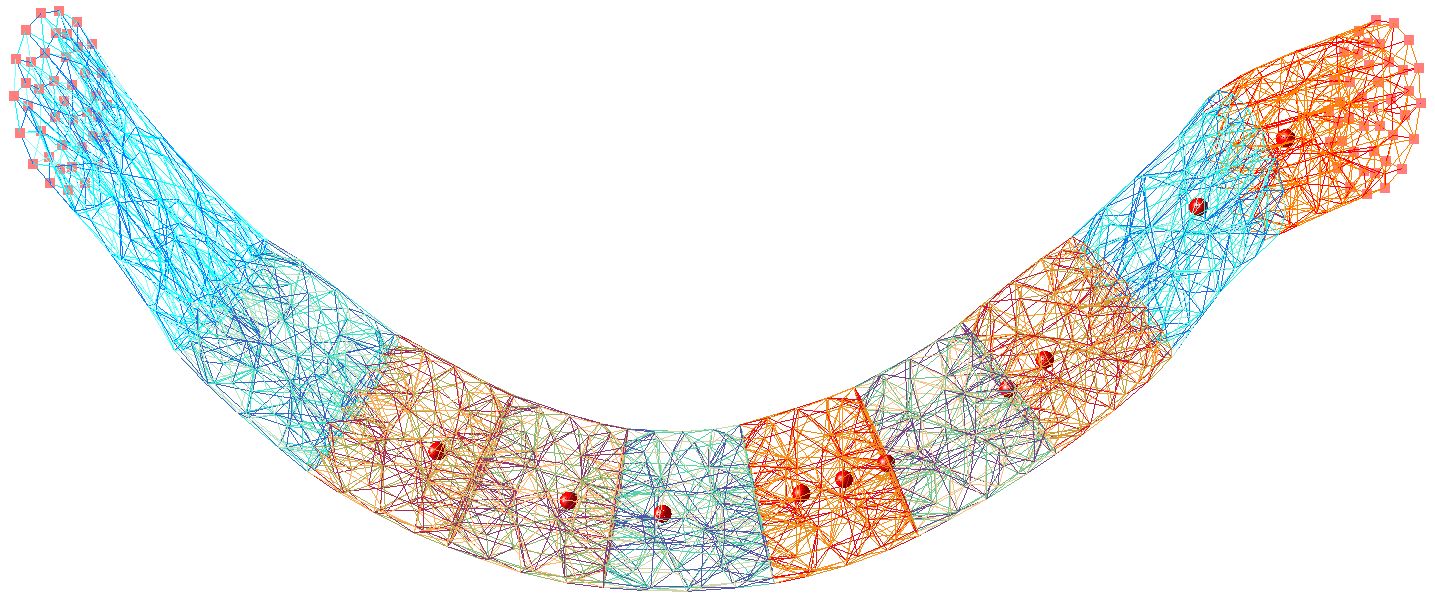
\includegraphics[width=.48\textwidth]{figs/cyl10screen.png}}
\caption{The cylinders used for the evaluation: (a) The mesh $\msa$ composed of 770 elements and 3 segments, with Young's moduli $\{8,2,10\}$\,kPa.
(b) The mesh $\msb$ composed of 4245 elements and 10 segments with Young's moduli $\{1,3,7,6,4,9,5,8,2,10\}$\,kPa}%
\label{f:cylScreens}
\end{figure*}

\section{Implementation}
\label{s:implement}

\subsection{Frameworks}
\label{si:frameworks}
In order to integrate the concepts of data assimilation based on reduced-order Kalman filtering, and the physics-based 
simulation of elastic deformations, we performed an integration of two frameworks. 

Simulation Open Framework Architecture (SOFA)~\footnote{\url{http://www.sofa-framework.org/}} is an open-source framework, written in C++. 
It primarily targets on the real-time simulation of deformable bodies and fluids, with an emphasis on medical simulation.
The framework allows for complicated simulation scenarios, benefiting from the possibility of creating complex 
scenes composed of hierarchically organized nodes populated by components. Each component represents a single functionality; for further details 
we refer the reader to~\cite{faure2012sofa}. It should be noted that a simulation in SOFA is always driven by an \emph{animation loop} 
which recursively calls visitors responsible for correct employment of different components. 

Verdandi~\footnote{\url{http://verdandi.sourceforge.net/}} is a generic, open-source library, written in C++. 
It aims at providing various methods and tools for data assimilation (DA) and currently consists of eight data assimilation methods
including EKF, UKF, ROEKF (a reduced-order variant of the EKF) and finally ROUKF. 
Verdandi is designed to be useful for a large variety of high-dimensional numerical models~\cite{chabiniok2012}. 

\subsection{Integration}
\label{si:integration}
Unlike a standard simulation where a new state is computed from the previous one by a single application of a model function (such as the one described in 
section~\ref{sm:model}), the data assimilation process based on the ROUKF presented in~\ref{sm:ROUKF} requires multiple evaluations 
of the model function, \ie\ it calls the model function with different parametrizations each corresponding to 
one sigma point. In order to perform the integration of SOFA (representing the model) and Verdandi (representing the driving filter), 
we have implemented a new animation loop which hands-over the control to the ROUKF. 
The filter executes the process described by Eq.~4 to 13 and it holds that
\begin{itemize}
\item In the prediction phase, it invokes a SOFA component called \emph{model wrapper} which is an abstraction of the SOFA functionality implementing the model function $f$ (Eq. 5) executed for each sigma point.
\item In the correction phase, it calls an \emph{observation manager} which implements the computation of innovation function $h$ (Eq. 8).
\end{itemize}
The scheme of the implementation is depicted in Fig.~\ref{f:integration}(a). 

\subsection{Parallel Sampling}
\label{si:parallel}
The algorithmic design of the ROUKF offers a great opportunity for parallelization of the sampling phase (evaluation of the model function 
for sigma points), as the task is embarrassingly parallel.
The parallelisation was implemented using Pthreads library which
appears to suit well the purpose and provides a performance at least similar to that of other options. 

The main issue related to the parellelization is given by the fact that unlike the sequential version where a single instance of the 
assimilated object is sufficient, the parallel version requires an independent instance for each thread. In reality, this 
means that at the beginning of the assimilation process, the simulation scene must be replicated so that $t-$ slave instances 
of the same object can be called independently by corresponding threads in order to evaluate the model function for given sigma point. 
The concept is presented in Fig.~\ref{f:integration}(b) where the model wrapper represent the same abstraction as before, however, it allows
 for multiple concurrent evaluation of the underlying simulation scene. 
 
 Since it cannot be assumed that the number of threads is equal to the number of sigma points, the evaluation of the model function 
 is assigned to the threads by a master thread. Since the workload performed by the slave threads can vary according to the number of
 processed sigma points and the length of computation of single model function, the threads are synchronized using a barrier at the end 
 of parallel sampling. The implementation is schematically depicted in Fig.~\ref{f:integration}(c). 









\section{Results}
\label{s:results}
In this section we present a preliminary evaluation of the proposed method dealing with the estimation of elastic parameters of a deformable 
object. The evaluation was performed using synthetic data which provide the ground truth that is used to assess the accuracy of the 
estimation. The section is structured as follows: first, we describe the testing scenarios used for the evaluation. Next, we 
present the quantified results demonstrating the accuracy of the estimations in terms of expected value and standard deviation. Finally, 
we focus on the performance of the actual implementation of the method. 

\subsection{Testing Scenarios}
\label{sr:scenarios}
The synthetic data used for the evaluation of the data assimilation technique allowing for the estimation of a large number of parameters
was generated using \emph{forward}, \ie\ a simulation executed for a given parametrization, based on the finite element corotational formulation of non-linear elasticity. 
Two tetrahedral meshes were generated for an object with cylindric shape using the Gmsh tool~\footnote{\url{http://geuz.org/gmsh/}}. 
The first mesh $\msa$ discretizing a cylinder ($l_1$=\SI{24}{\cm} and $r_1$=\SI{2}{\cm} being the length and radius) 
is divided into three segments and consists of 770 elements; the second mesh $\msb$ represents a domain of cylinder 
with $l_2$=\SI{30}{\cm} and $r_2$=\SI{2}{\cm}, divided into 10 segments composed of 4245 elements in total. 

Both meshes are first employed in the forward simulation using SOFA as follows: each cylinder is fixed on the lateral facets
using homogeneous Dirichlet conditions and the gravity is applied to the object having density $\rho$ = \SI{1000}{\kg\per\cubic\metre}.
The behavior of each cylinder is modeled with corotation finite element formulation. While constant Poisson's ratio ($\nu$ = \SI{0.45})
is applied over the entire volume of both cylinders, different Young's modulus is attributed to each segment mimicking the 
heterogeneous nature of tissues. 
The simulation is performed using quasi-static solver where in each step, the gravity is increased by 1/100 of the target value, 
thus requiring 100 steps to reach the final deformation. Single linearization per simulation step is performed and the 
linearized system of equations is factorized using LDL solver Pardiso~\footnote{http://www.pardiso-project.org/}. 
In each step, the actual position of all nodes is stored in a file which later serves as the source of observations. The deformed configurations are depicted in Fig.~\ref{f:cylScreens}. 

\begin{figure*}[th]%
\centering%
\subfigure[]{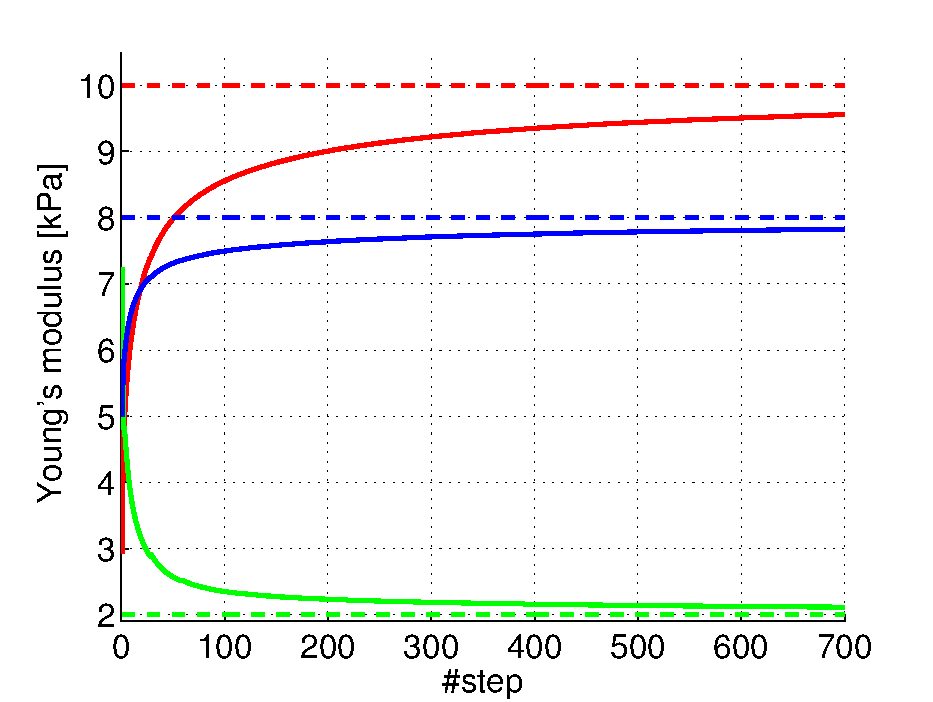
\includegraphics[width=.32\textwidth]{figs/cyl3_par.pdf}}
\hfill
\subfigure[]{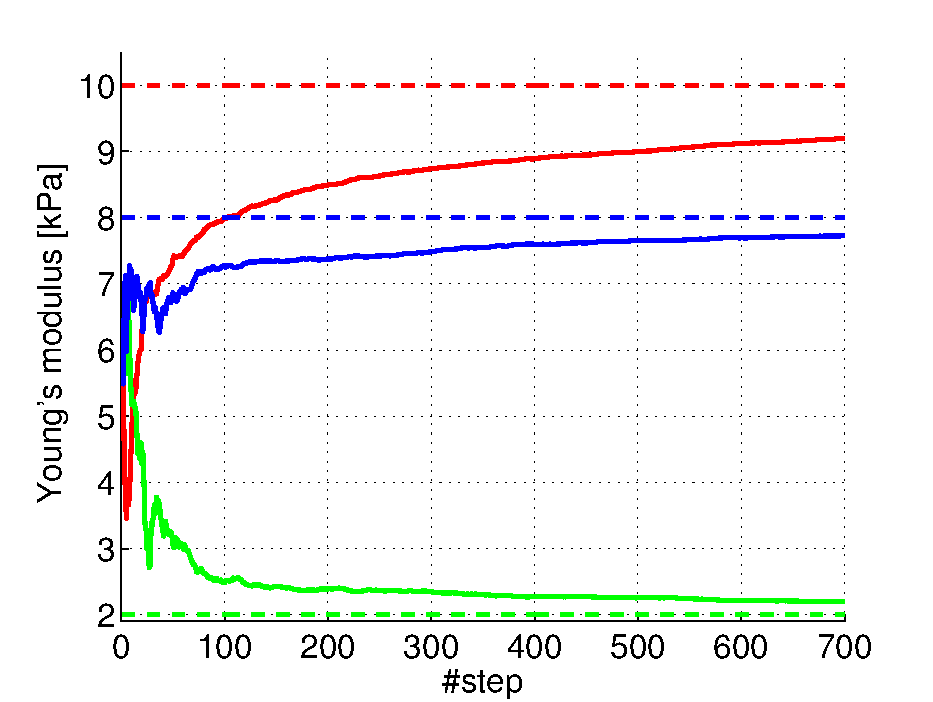
\includegraphics[width=.32\textwidth]{figs/cyl3ns_par.pdf}}
\hfill
\subfigure[]{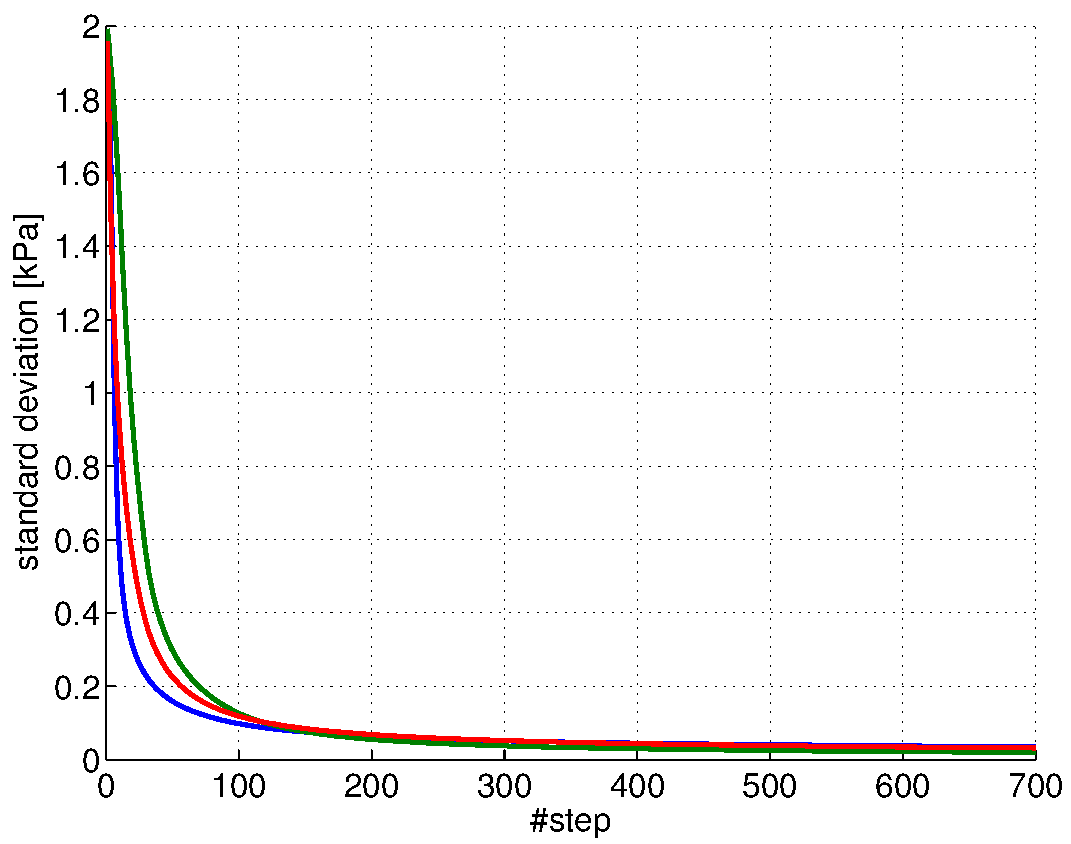
\includegraphics[width=.32\textwidth]{figs/cyl3ns_var.pdf}}
\caption{Results of the estimation of parameters for $\msa$: Three parameters are estimated, each associated to 
one segment. Figures (a) and (b) show the evolution of the parameter estimation as the function of the quasi-static 
incremental gravity loading without and with noise added to the observations, respectively. The dashed lines indicate the ground-truth 
and the estimation starts in the undeformed configuration. The plot (c) shows the evolution of standard deviation 
associated to each parameter and their combinations, respectively.}
\label{f:cyl3Estim}
\end{figure*}

\begin{figure*}[t!]%
\centering%
\subfigure[]{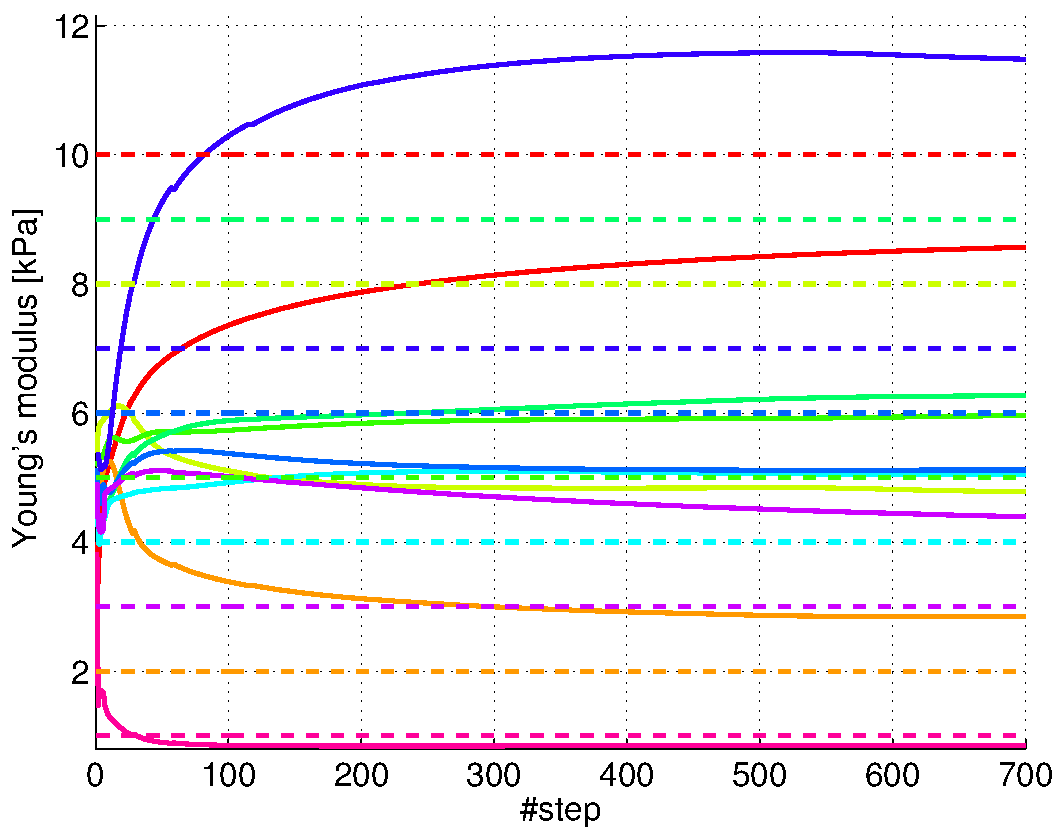
\includegraphics[width=.32\textwidth]{figs/cyl10_par.pdf}}
\hfill
\subfigure[]{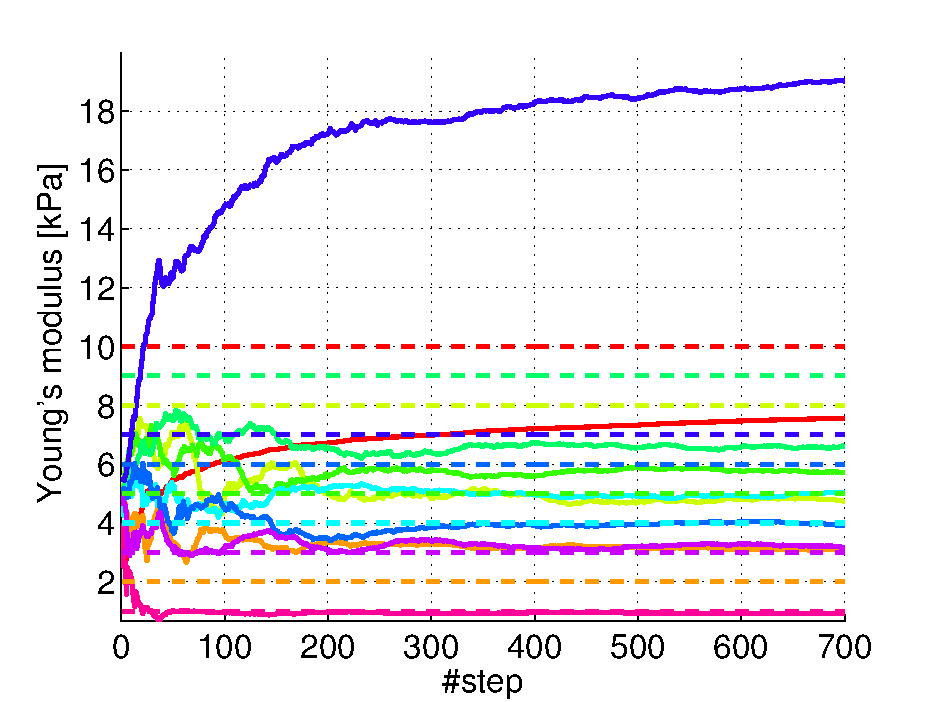
\includegraphics[width=.32\textwidth]{figs/cyl10ns_par.pdf}}
\hfill
\subfigure[]{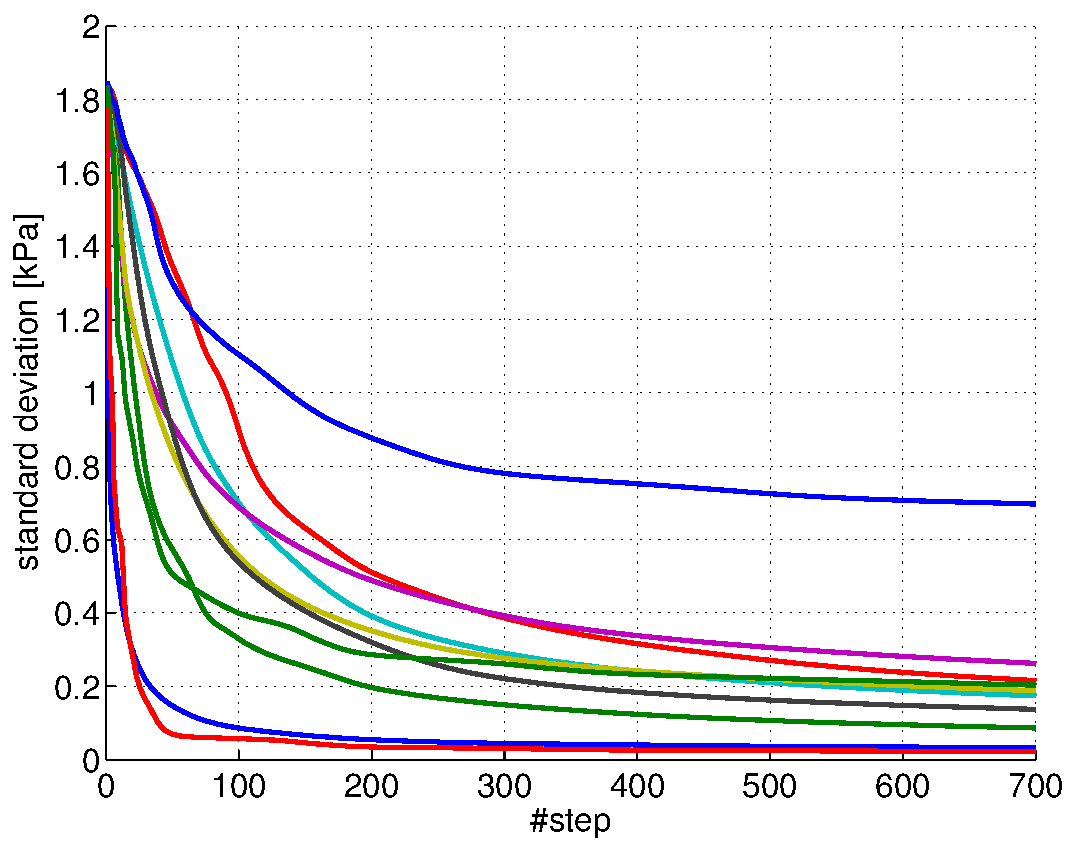
\includegraphics[width=.32\textwidth]{figs/cyl10ns_var.pdf}}
\caption{Results of the estimation of parameters for $\msb$: Ten parameters are estimated, each associated to 
one segment of the mesh. Figures (a) and (b) show the evolution of the parameter estimation as the function of the quasis-static 
incremental gravity loading without and with noise added to the observations, respectively. The dashed lines indicate the ground-truth 
and the estimation starts in the undeformed configuration. The plot (c) shows the evolution of the standard deviation 
associated to each parameter and their combinations, respectively.}%
\label{f:cyl10Estim}
\end{figure*}

\subsection{Parameter estimation}
\label{sr:estim}
The parameter estimation was performed using the ROUKF method described 
in section~\ref{sm:ROUKF} employing the implementation based on the SOFA and Verdandi frameworks. 
Two different reconstruction scenarios were tested: first, for both $\msa$ a $\msb$, the number of parameters to estimate was 
set to the number of segments, \ie\ 3 and 10 parameters each corresponding to the value of the Young's modulus of the respective segment. 
At the beginning of each estimation, the same expected value $\eexp$=\SI{6000}{\Pa} and standard deviation $\evar$=\SI{2000}{\Pa} was attributed to 
each estimated parameter. This means that the information about geometrical distribution of the heterogeneous segments was 
given as \emph{a priori} known assumption and the data assimilation was used to estimate the parameter of given pre-defined segment.

In the second scenario applied only to the mesh $\msa$, no assumption about the distribution of the heterogeneous regions was made. 
Therefore, it was necessary to consider the Young's modulus of each element as an independent parameter. Given the size of the 
mesh, 770 parameters were to be estimated by the ROUKF method.  

The correction phase of the assimilation process is directly determined by the computation of the innovation based on observations.
Given the quasi-static scenario, only positions are used as the observed quantities. 
Nevertheless, instead of using all known positions (\ie\ position of all the nodes 
in $\msa$ and $\msb$), we limited the observations to 10 points located on the axis of each cylinder as shown in Fig.~\ref{f:cylScreens}. 
Therefore, the Kalman gain computed by the ROUKF calculates the innovation using the actual Euclidean distance between the position of 10 points 
mapped to the actual deformed configuration of the cylinder estimated by the data assimilation process, and the real positions of 
the points computed from the synthetic observation data generated during the forward simulation. In order to mimic the 
real scenarios where the observations usually suffer from noise, the elements of the observation vectors were modified using 
Gaussian white noise with standard deviation $\text{Var}_\text{noise}$ = \SI{2}{\mm}.



\begin{figure*}[t!]%
\centering%
\subfigure[]{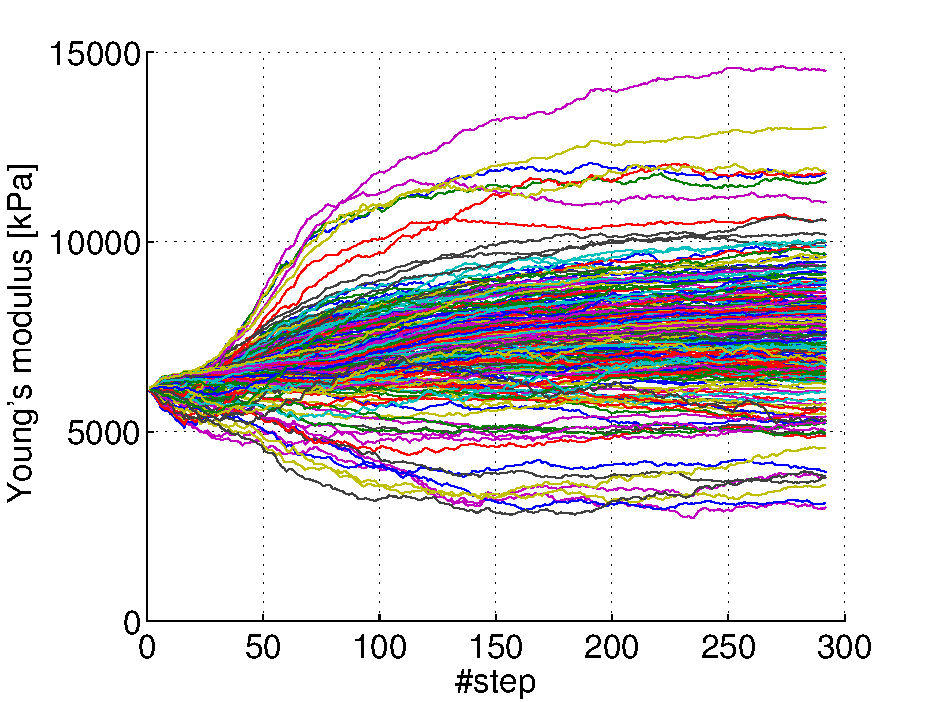
\includegraphics[width=.32\textwidth]{figs/cyl3EA_seg3.pdf}}
\hfill
\subfigure[]{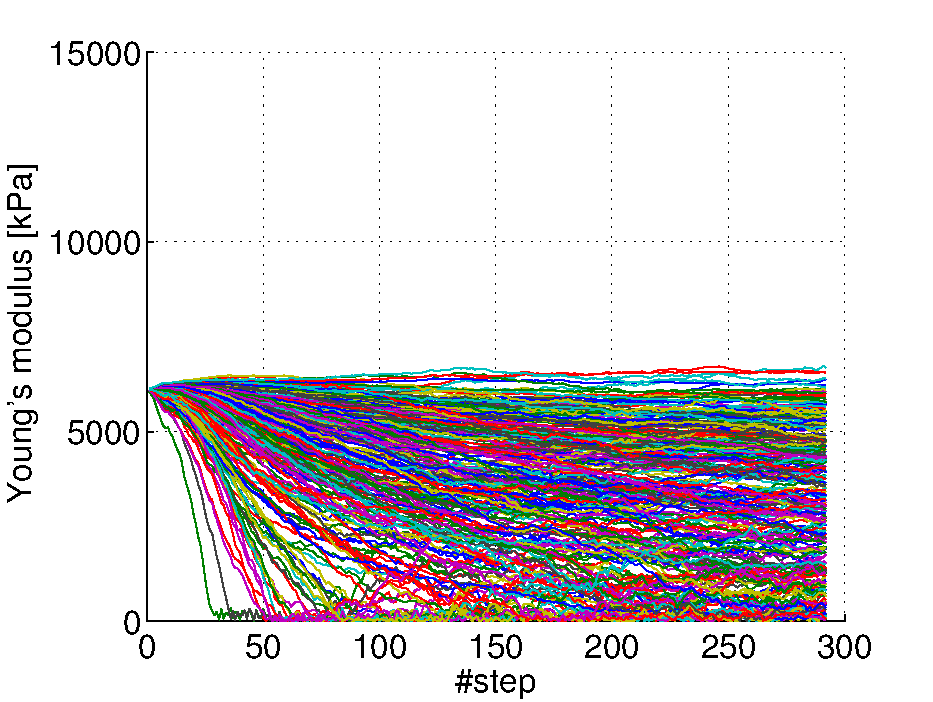
\includegraphics[width=.32\textwidth]{figs/cyl3EA_seg2.pdf}}
\hfill
\subfigure[]{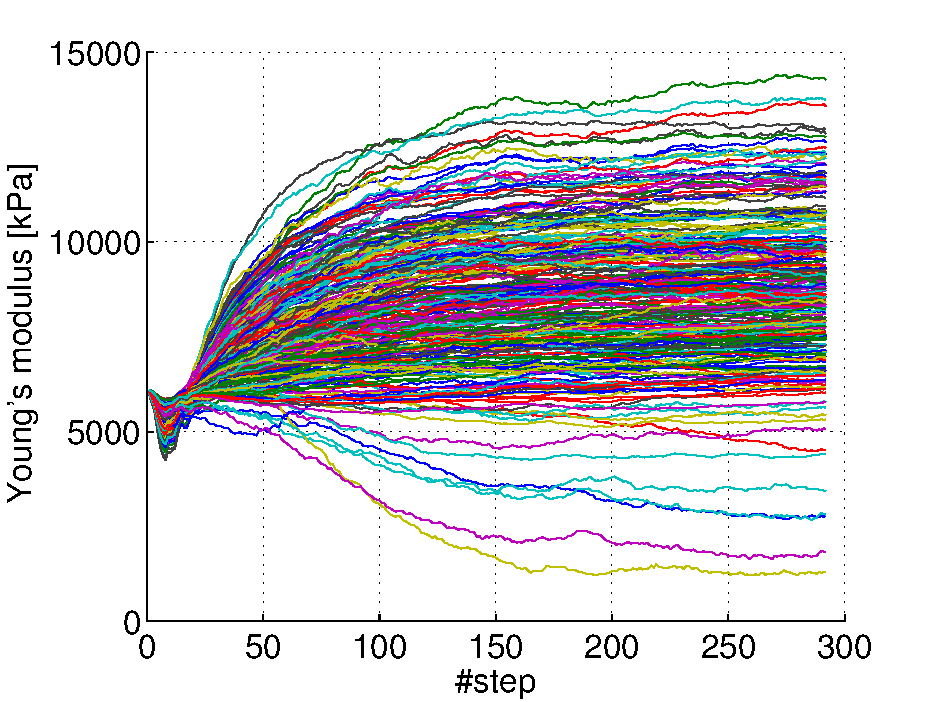
\includegraphics[width=.32\textwidth]{figs/cyl3EA_seg1.pdf}}
\caption{Evolution of the elasticity estimation independently for each element as functions of the quasi-static incremental gravity loading.
The three plots (a), (b) and (c) shows the evoluation of estimations associated to elements from segment 1, 2 and 3. We recall that 
the Young's moduli used in the forward simulations were $\{8,2,10\}$\,kPa}.%
\label{f:cyl3EAsegs}
\end{figure*}


\subsection{Estimation of Elastic Modules per Segment}
\label{sr:segment}
The results obtained for the estimation of elastic modules associated to each segment are presented in Fig.~\ref{f:cyl3Estim} for 
$\msa$ and in Fig.~\ref{f:cyl10Estim} for $\msb$. In the case of $\msa$, the estimated expectations converge to the real values 
used in the forward simulation even with added noise. This is also reflected by the fact that the standard deviation associated to each 
parameter quickly approaches zero. In the case of $\msb$, the situation is more complicated as for some parameters, the convergence is clearly 
not achieved. However, these parameters can be identified (without knowing the ground-truth) from the respective standard deviation which 
remain important event after large number of steps, thus indicating significant uncertainty associated with the estimation. 
Nevertheless, given the limited number of the observation points which is equivalent to the number of estimated parameters, 
the results signal an interesting level of robustness of the estimator. 

\subsection{Estimation of Elastic Modules per Element}
\label{sr:element}
In this evaluation, the elasticity of each element of the mesh $\msa$ was estimated as an independent parameter. Thus, 770 parameters were estimated in total. 
The expected values were stored in each step of the data assimilation process. In order to facilitate the visualization, 
the histories of parameter estimations were plotted separately for each segment as shown in Fig.~\ref{f:cyl3EAsegs}. 
It should be emphasized that the curves were regrouped \wrt\ the segments as a part of data post-processing and so no \emph{a priori} 
information about the location of given element \wrt\ the segments was given during the data assimilation process. 
In order to get more quantitative assessment, Fig.~\ref{f:cyl3EAmeans} shows the mean curves computed for each segment 
from Fig.~\ref{f:cyl3EAsegs}. The preliminary evaluation suggests that the data assimilation based on ROUKF is capable of 
reliable estimation of the elasticity parameters even for the somewhat extreme case where the elasticity of each element of the 
mesh is treated as an independent parameter to be estimated. For the sake of clarity, we are not plotting the standard deviation
of the parameters, however, we plan to perform statistical evaluation of these quantities which is beyond the scope of this paper. 

\subsection{Performance of the method and parallelization}
\label{sr:perf}
The performance of the method was evaluated using a single cluster node equipped with 16 CPUs AMD Opteron 6274 running at \SI{2.2}{\giga\hertz}.
The procedures were executed at least 3 times and mean measured value is reported. 
In order to quantify the performance of the data assimilation, we first report the performance of the 
forward simulation: in the case of $\msa$, the forward simulation in SOFA was running at \SI{50}{FPS} while the data assimilation using the 
\emph{simplex} type of the sigma points was running at about \SI{20}{FPS}. Similarly, the direct simulation using $\msb$ 
was running at \SI{20}{FPS}. In this case, the data assimilation was much slower: the refresh rate did not exceeded \SI{1}{FPS}. This 
is however expected due to larger number of parameters to be estimated.

As for the scenario where the elastic modules were estimated per elements, the running time is significantly longer: one step of the data assimilation 
took about 15 s for the simplex, and 25 s for the star type of the sigma points. 

The numbers reported above were measured for the sequential execution of the data assimilation. The impact of the parallelization 
is depicted in Fig.~\ref{f:parallel} where the estimation of 10 parameters using the mesh $\msb$ was executed using 1, 4, 8, 12 and 16 threads
for all the three types of the sigma points. Since the parallelization was performed only for the predictive case, the plot 
indicates the limits this approach, since even for the \emph{star} ROUKF, no speed-up is observed when the number of threads exceeds 12, 
despite the fact that the model step (performed in parallel) was executed 21 times. 

%\input{discussion.tex}
\begin{figure}[t!]%
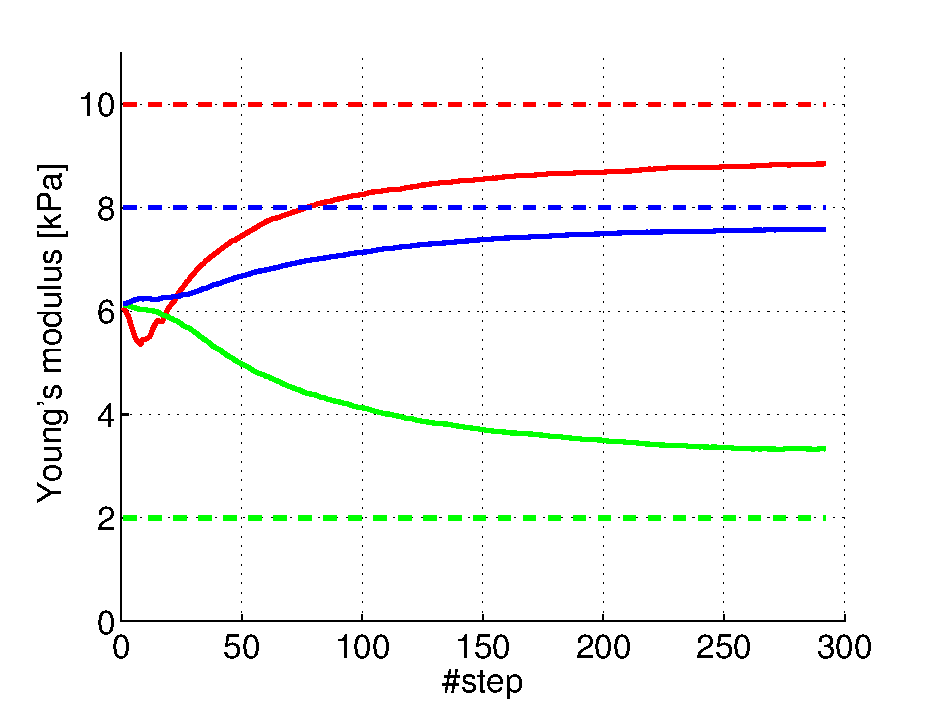
\includegraphics[height=6cm]{figs/cyl3EA_means.pdf}
\caption{The evolution of the average elastic modules computed as the mean over the element belonging to segment 1 (blue), 2 (green) and 3 (red), 
\ie\ each curve represent a mean of curves plotted in Fig.~\ref{f:cyl3EAsegs} (a), (b) and (c), respectively.}
\label{f:cyl3EAmeans}
\end{figure}

\section{Conclusion and Perspectives}
\label{s:conclusion}
In this paper, we have demonstrated that it is possible to bridge the gap between the world of physically-based models 
and the domain of data assimilation methods based on Kalman filtering. We have employed a state-of-the-art  
\emph{reduced-order unscented Kalman filter} to estimate the Young's modulus in heterogeneous object modeled by 
the co-rotational formulation of non-linear elasticity. 
%The method was based on integration of two 
%packages, SOFA and Verdandi, which was in turn employed in different scenarios as described in section~\ref{sr:scenarios}. 
We have performed an experimental estimation of system with 770 parameters; although the approach requires further 
evaluation, the preliminary results are encouraging as they suggest significant reliability and robustness of the estimator. 

We are aware of the fact that the method was evaluated using only the synthetic data which where moreover generated using 
the FE model identical to the one used in the estimation.
At the same time, we believe that the initial testing requires knowledge of the ground-truth which is
usually available only for synthetic data. 

%As the next step, we want to focus on the correction phase, so that it would allow for integration 
%of the data assimilation technique with a real-life object with known mechanical properties. 

In the near future, we plan to further improve the performance of the method. As demonstrated in section~\ref{sr:perf}, 
the parellelization of the prediction phase has brought only limited improvement, as the mathematical operations 
performed by the filter itself has become increasingly expensive, especially with growing number of parameters. 
We have already performed a code profiling in order to identify the actual bottlenecks of the algorithm. 
Since the filter manipulates mainly with the stochastic data such as the co-variance dense matrices, we have
performed a preliminary estimations showing that employing GPGPUs would resunt in a significant acceleration.
We are also working on employment of the actual version of the algorithm in real scenarios of medical planning and navigation.

\begin{figure}[t!]%
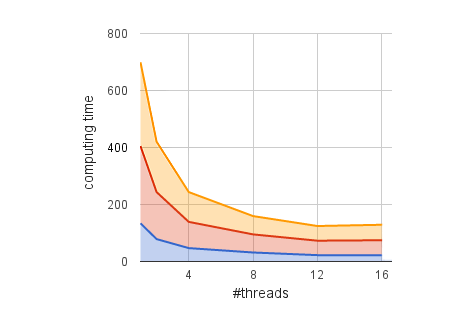
\includegraphics[height=6cm]{figs/cyl10parallel.png}
\caption{The impact of the parallelization on the computation time in [s] needed to perform 100 steps of the data assimilation used for 
the estimation of 10 parameters on mesh $\msb$. Three different types of sigma points were tested: \emph{simplex} (blue curve), 
\emph{canonical} (red curve) and \emph{star} (yellow curve).}
\label{f:parallel}
\end{figure}


%\enlargethispage{1mm}
\bigskip

\bibliographystyle{IEEEtran}
\bibliography{biblio}



% that's all folks
\end{document}


